\chapter{物理量と単位}\label{chapt:dim_unit}
%{\small 君は「はじめに」を全部, 隅々まで読みましたか? 
%読まずに進むと, 誤った方法で勉強することになり, 時間と努力を無駄にします。}\\

\section{物理量は, 数値×単位}\label{sect:dimension}

数学は数を抽象的な概念として扱う。例えば数学で
「方程式$3x=x+4$の解は$x=2$である」
という時の$x=2$は, 何か具体的なものの量を想定してはいない。

一方, 現実の様々な問題では, 何らかの実体を伴った具体的な量
を扱う。例えば「君の身長」や「君の100~m走の記録」は
具体的な実体を表す量である。このように, 具体的な実体を
表す量のことを\underline{物理量}\index{ぶつりりょう@物理量}
と呼ぶ\footnote{物理が嫌い!苦手!という人もいるが, 
世の中の量のほぼ全ては「物理」量であり, その計測や扱い
において, 物理学の考え方は必要である。}。

物理量は, 通常, 160 cmとか12.3 秒というふうに, 数値と単位の
積(掛け算)で表される。君は160 cmというとき, 
cmという単位は, 160という数値のオマケか添え物のように
思っているかもしれないが, そうではない。160 cmとは
\begin{eqnarray}
160 \times\text{ cm}
\end{eqnarray}
という意味だ(積を表す$\times$は省略されている)。
つまり, 160 cmは, 「cm(センチメートル)を160個
ぶん集めた量(長さ)」だ。同様に, 12.3秒とは
$12.3\times$秒であり, 「秒を12.3個ぶん集めた量(時間)」
だ。このように, 物理量の大きさは
「何の何個分」という形で表され, その「何の」に相当する
のが\underline{単位} (unit)\index{たんい@単位}である
\footnote{「単位」は多義語であり, 大学の授業をいくつ
履修したか(英語では"credit")を表する時も使う。}。

物理量の扱いで, 数値が正しくても単位を間違えると大惨事になる。

\begin{exmpl} 1999年9月23日, 米国の火星探査機
「マーズ・クライメート・オービター」が, 火星に到達した
直後に, 消息を断った。探査機を制御する2つのチームが, 
片方はメートルやキログラムという単位を使い, もう片方は
ヤードやポンドという単位を使っており, データ共有に失敗して, 
制御不能で事故に至ったらしい。\end{exmpl}

\begin{exmpl} 2000年3月30日, 埼玉県川口市の病院で, 
ある患者が, 薬剤を過剰投与され, 死亡した。
医師の指示では薬剤は80 mgだったが, 処方箋には, 
80アンプルと記入され(1本のアンプルには10 mgの薬剤が入っている), 
結果的に, 看護師が800 mgの薬剤を投与したらしい。(例おわり)\end{exmpl}

しかし, 大変残念ながら, 伝統的に, 生物資源学類生の多くは, 
単位が苦手であり, 単位を平気で付け忘れる\footnote{その一部は, 
単位に自信がないから, 「つけ忘れたふり」をしてごまかしてるのだろう。}。
当然, そのような答案は不正解であり, 0点である。いにしえの資源生曰く, 
「\textgt{単位(unit)を忘れて単位(credit)を落とす}」と。

\begin{faq}{\small\textgt{そこまで単位にこだわらなくても
いいのでは?} ... 
君が農家で, 単位を間違えて基準を超える濃度で農薬撒いたら
どうなります? 野菜全部出荷停止ですよ。}

%\begin{faq}{\small\textgt{そういうシリアスな状況では, 
%もちろんちゃんと単位つけますよ。} ...
%そんなこという人の野菜なんか, 怖くて誰も買いませんよ。
%大切なことは, 普段から気をつけて習慣にしておかないと, 
%いざというときにミスするのです。}\end{faq}

{\small\textgt{でも, 高校や, 大学でも他の授業では, 
単位の付け忘れは減点だけです。0点なんて, 厳しすぎませんか?}
... そんなぬるい教育をするから大惨事が起きるのです。}

{\small\textgt{でも, 「三角形ABについて
辺ABの長さを$1$とする」みたいに, 最初から単位が無い
問題文もあるじゃないですか? }
... 数学でよくあるそういう問題は, 
ABの長さが1~cmであっても, 1~mであっても, 1~kmであっても
通用するように作られているのです。こういうときは
答にはもちろん単位をつける必要は無いし, つけてはダメ。}

{\small\textgt{物理でも, 「力を
$F$とし, 質量を$m$とする...」みたいに, 単位が書かれて
いない問題がありますよね?} ... 単位はその$F$や$m$の
\textgt{中に}含まれているのです。例えば$m$を実際に
数値で表すと, 「$m=3$~kg」や「$m=3000$~g」
と書いたりします。このとき, $m$には, 3や3000という数値
だけでなくkgやgという\textgt{単位も一緒に入っている}のです。}

{\small\textgt{「$t$秒の時間で, 
毎秒2~mの速さで, 6 m進んだ。$t$を求めよ」みたいな問題は? 
「$t=$3 秒」ですか?「$t=$3」ですか?} ... 問題文で, 
その時間は「$t$かける秒」で定義されている(単位は
変数$t$の外に出されている)ので, $t$は単位を持って
いません(後述する無次元量)。従って$t=3$が正しいです。
でもこういう書き方は稚拙であり, 大学では一般的ではありません。
}\end{faq}

さて, 複数の物理量どうしを足したり引いたり, 大小を比べたりするには, 
単位を揃える必要がある。例えば, 「20 cm + 1.23 m=?」という問は, 
\begin{eqnarray}
&&0.2\text{ m} + 1.23\text{ m} = 1.43\text{ m}\label{eq:0.2m+1.23m}\\
&&20\text{ cm} + 123\text{ cm} = 143\text{ cm}\label{eq:20cm+123cm}
\end{eqnarray}
というふうに, ひとつの単位に揃えないと計算できない。また, 
20 cmと1.23 mのどちらが大きいか? という問に, 20と1.23という
数の大小だけで判断して「20の方が大きい!」というのは愚かである。

こういう話をアタリマエだ! と思わずに, よく考えよう。
\eref{eq:0.2m+1.23m}を丁寧に考えれば, まず左辺の2つの
項をmという量でくくって, 左辺=(0.2 + 1.23) m
という式を立て, その括弧内を普通に数どうしの足し算で計算し, 
右辺の1.43 mに至るのだ。この「共通する量でくくる」ところで, 
暗黙のうちに分配法則(\eref{eq:axiom_num_distr})を逆向きに
使っているのだ! それは, 0.2~mや1.23~mという量を, ともに
「同じ単位の何倍か」に揃えたからできたのだ。改めて, 
単位は単なる添え物ではなく, 物理量の重要な一部だと感じられ
るではないか!\mv

\section{次元}

さて, どんなに頑張っても単位を揃えられないような量どうしも
存在する。例えば20 cmと5 時間がそうである。前者は長さ, 
後者は時間を表すのだから, 単位は揃えられない。

こう考えれば, 世の中の様々な物理量は「互いに単位を
揃えられるかどうか」という観点で分類できるだろう。
そういう性質を「\underline{次元}」\index{じげん@次元}
と呼ぶ。上の例では, 20 cmという量は「長さ」という次元を持ち, 
5 時間という量は「時間」という次元を持つ。\mv

\begin{q}\label{q:alg_dim00} (本節で出てきた)次元とは何か?\end{q}

次元が違う量どうしは, 足したり引いたり, 大小を比較したり
はできない。実際, 20 cmと5 時間を「足す」ことはできないし, 
無理に20と5を足して25を得ても, それはもはや何の物理量も
表さない。「20 cmと5 時間はどちらが大きいか」などという
問も無意味である。\\



\section{単位の掛け算と割り算}\label{sect:unit_mult_div}

ところで, 単位は, 普通の数と同じように掛け算ができる:

\begin{exmpl} 隣接する2辺の長さが2 mと3 mで
あるような長方形の面積は, 
\begin{eqnarray}
2\text{ m}\times3\text{ m}=6\text{  m}^2\label{eq:rect_area00}
\end{eqnarray}
である。このとき, 結果にm$^2$という単位が出てきたのは, 
「面積を求めたから」というよりも, 「mを2回掛けたから」
なのだ。(例おわり)\end{exmpl}

単位は, 割り算もできる:

\begin{exmpl} 100 mの距離を20 秒で走る人の(平均の)速さは, 
\begin{eqnarray}
\frac{100\text{ m}}{20\text{ 秒}}=5 \text{ m}/\text{ 秒}\label{eq:100m20s_speed}
\end{eqnarray}
となる。このとき, 単位どうしの割り算の結果として, 
速さの単位「m/秒」が出てきた。\textgt{この単位の/という
記号は, 割り算の記号}なのだ。従って, m/秒を$\frac{\text{m}}{\text{秒}}$
と書いてもOKである。(例おわり)\end{exmpl}

\begin{faq}{\small\textgt{割算に/という記号をなるべく使わない, 
という約束がありましたが, m/秒はOKなのですか?} ... 
慣習的に, 単位の中では/をよく使います。例外ということに
しておきましょう(国際規格でも認められている)。}\end{faq}

「5~m/秒」は「5メートル毎秒」とか「毎秒5メートル」とも言われる。
このような「毎...」は, 「...という単位あたり」と同じ事である。
「5メートル毎秒」は「1秒あたり5 m」と同じである。
そして, 「...あたり」は「...で割る」という意味である。たとえば, 
「りんご6個を3人でわけるとき, 一人\textgt{あたり}いくつ?」
という問には, 6個$\div$(3人)で計算するだろう。

困ったことに, 世の中にはこの「毎...」や「...あたり」を省略するという
悪習がある。決して真似てはいけない。

\begin{exmpl} 日本のGDP(国内総生産)は, 1人あたり約4万ドルと
言われることがある。これは, 1人あたり\underline{1年間あたり}
約4万ドル, もしくは約4万ドル/(人・年)が正しい。\end{exmpl}

\begin{exmpl} テレビの天気予報では, 「台風の中心付近の
最大瞬間風速は40~m」などと言われるが, これは\underline{毎秒}40~m, 
もしくは40~m/秒が正しい。\end{exmpl}

\begin{exmpl} 放射線量を表すときに使われるSv (シーベルト)
とSv/h (シーベルト毎時)は全く違う単位なのに, 
後者を省略して前者のように言ってしまう報道が多い。
これはヤバイ。例えば1~$\mu$Sv/hと1~$\mu$Sv/sは, 
/hや/sを省略したら同じ表現になってしまうが, 実際は, 
後者は前者の3600倍である。(例おわり)\end{exmpl}\mv

こういう悪習を人前で晒すと恥をかく。その恥は, 本人だけ
でなく, 出身大学まで及ぶ。

ここまで読んで, 君は「面倒くさ!」と思ってる
かもしれないが, 単位は君を助けてくれることもある。
次節では小学校レベルの問題を扱うが, 意外に苦手な人も多い。
そういう問題で, 単位が役に立つのだ。\\

\section{単位を埋め込んで計算せよ!}
ところで, \eref{eq:rect_area00}を, 次のように書く人が多い:
\begin{eqnarray}
2\times3=6\text{  m}^2\label{eq:rect_area00_NG}
\end{eqnarray}
高校の参考書もこういう記法を勧めてたり, 大学教員にもこう書く
人がいるが, これは変だ。なぜか? もしこういう書き方がOKなら, 
「2辺の長さが2~cmと3~cmの長方形の面積は?」という問題についても, 
\begin{eqnarray}
2\times3=6\text{  cm}^2\label{eq:rect_area00_NG2}
\end{eqnarray}
と書けるはずだ。\eref{eq:rect_area00_NG}と\eref{eq:rect_area00_NG2}の
左辺は共通なので, 等号の公理(\eref{eq:equality03})から, 
\begin{eqnarray}
6\text{  m}^2=6\text{  cm}^2\label{eq:rect_area00_NG3}
\end{eqnarray}
\textgt{これは明らかに変だ!} その原因は, 
\eref{eq:rect_area00_NG}と\eref{eq:rect_area00_NG2}の
左辺に単位を埋めこまなかったことにある。\textgt{単位を持つ量
の計算は, 式の中に数値だけでなく単位も埋め込む}べきなのだ。
そうすれば, 単位の誤記や, 単位のつけ忘れという重大なミスを
防止できる。\mv

式の中に単位を埋め込みたくなければ, \eref{eq:rect_area00_NG}
や\eref{eq:rect_area00_NG2}の右辺の単位も書かなければよい。
それは, 単位を外した数値\footnote{それは後述する「無次元量」である。}
の間の計算であり, 論理的には問題ない。そして出てきた数値に改めて
単位をつけた答を, 別の場所に書くのだ。それもめんどくさい人は, 
\begin{eqnarray}
2\times3=6\quad\quad\text{[m$^2$]}\label{eq:rect_area00_NG5}
\end{eqnarray}
と書いたりする。この場合, 右の方の[m$^2$]は, 「最後に出てきた数値に
この単位を掛けたものが, 最終的な答えですよ」という事情を書き添えた
「メモ」であり, 等式の一部ではない。

しかし\textgt{これらはいずれも不合理な慣習である}。やはり単位を埋め込んで
計算すべきなのだ。そうすれば, \textgt{単位が計算を助けてくれる}ことがあるのだ。\mv

\begin{exmpl}\label{exmpl:niku600yen} 120~gで600円の肉は, 900~gでいくらか? 
もちろん, 「120~gあたり600円」だから1 gあたり... と考えて, 
ここは割り算, ここは掛け算, というふうに進めてもいいが, 
単位を頼りに考えると楽なのだ:
\begin{eqnarray}
\frac{600\text{円}}{120\text{ g}}\times 900\text{ g}=
\frac{600\times900}{120}\frac{\text{円}\teisei{\text{ g}}}{\teisei{\text{ g}}}
=4500\text{ 円}\quad\quad\quad\label{eq:mihaji02}
\end{eqnarray}
\eref{eq:mihaji02}の左辺には, それぞれの数値に単位をつけた。
つまり, 単位を式に埋め込んだ。数値と単位は掛け算の関係なので, 
順番を入れ替えて, 数値の計算と, 単位の計算に分離する。
そして数値は数値で計算し, 単位は約分して簡単にする。
そうすれば, 最後に「円」という欲しかった量の単位が現れ, 
立式が正しかったことが裏付けられる。
もしもこの問題を, うっかり
\begin{eqnarray}
\frac{120\text{ g}}{600\text{円}}\times 900\text{ g}=...\label{eq:mihaji04}
\end{eqnarray}
とやっちゃったら, 最終的な単位がg$^2$/円になる。
これは意味不明なので, 何か間違っていた, とわかるのだ。\end{exmpl}

\begin{exmpl}\label{exmpl:mihaji} 小学校で, 速さと道のりと時間の関係を, \\
 「速さ=道のり$\div$時間」\\
 「道のり=速さ$\times$時間」\\
 「時間=道のり$\div$速さ」\\
と習った。これを, いわゆる「みはじ」, つまり
\begin{eqnarray}
\frac{\text{み}}{\text{は }|\text{ じ}}
\end{eqnarray}
という図式(「み」は道のり, 「は」は速さ, 「じ」は時間)で
覚えた人も多いだろう(「みはじ」以外にも「きはじ」とか
「はじき」とか「木の下にはげ爺さん」などのバージョンもあるらしい)。
しかし, このような図式を忘れても, 単位をチェックすれば
正しく計算できる。実際, 速さをm/秒, 道のりをm, 時間を秒
で表すならば, 例えば速さ3~m/秒で時間5秒だけ走るときの道のりは, 
単位も埋め込んで正しく計算すれば\\
\begin{eqnarray}
3\frac{\text{m}}{\teisei{\text{秒}}}\times 5\teisei{\text{秒}} = 15\text{ m}\label{eq:mihaji06}
\end{eqnarray}
となり, 無事に距離の単位mが出てくる。ところが, これを
割り算にしたりすると, m/秒$^2$や秒$^2$/mという, 変な単位
が出てくる。そういう変な単位にならないように, すなわち, 
目標とする単位が最終的に残るように立式すればよいのだ。(例おわり)\end{exmpl}

「速さ, 道のり, 時間」のように, 互いに積や商の関係
にあるような3つの量を処理するという状況は, 他にも
たくさんある。それらのひとつひとつに
「みはじ」みたいなのを考えるのはきりがない。
単位を埋め込んで, 単位を手がかりに処理すればいいのだ。
\mv

\begin{faq}{\small\textgt{でも, このやりかた, めんどくさいです。} ... 
私も最初はそうでした。でも, 結局はこの方が正確で便利なのです。
数値だけの計算だと, ミスしやすいのです。ミスの発見と修正には
多くの時間が必要ですからね。それに, 学校のテストならミスは
減点だけですが, 仕事でのミスは大事故や大損害になりかねません。}\end{faq}
\mv

\begin{q}\label{q:unit_mihaji} 以下の問を, 単位を式の中に埋め込んで解け。
\begin{enumerate}
\item 5時間で500リットルの水が出る蛇口から2時間で流れ出る水の量を求めよ。
\item 5時間で500リットルの水が出る蛇口から4~m$^3$の水を出すのに,どのくらいの時間がかかるか?
\item つくば市の水田面積は約4900~ha, コメの収穫は年間21,000~tである(つくば市ホームページ)。つくば市の水田は1年間で, 
単位面積あたり, どのくらいのコメがとれるか? kg/m$^2$という単位で答えよ。
\item つくば市で, 単位質量のコメの生産に必要な水田の面積を求め, m$^2$/kgという単位で答えよ。
\item 筑波大学の筑波キャンパスは, 約260万m$^2$である。これと同じ面積の水田をつくば市で借りたら, 
年間何トンのコメがとれるか?
\item 日本の成人1人は年間約60~kgのコメを消費する。生物資源学類1年生約130人の消費するコメを
つくば市の水田だけでまかなうなら, どのくらいの面積の水田が必要か?
\item タイのある農村に, 面積120~haのキャッサバ農地がある。ここで毎年収穫されるキャッサバの総額は日本円で概ねいくらか? ただし, 当地方のキャッサバ農地では毎年, キャッサバは1ライあたり平均約2.5トン収穫されることが別の調査でわかっている。ライというのはタイで使われる面積の単位で, 1ライは1600~m$^2$である。また, キャッサバの市場価格は4.4バーツ/kgである。バーツというのはタイの通貨単位で, 100円が33バーツである。
\end{enumerate}
\end{q}



\section{無次元量}

ところで, 同じ次元を持つ量どうしの割り算は, 面白い結果になる。
例えば, 直径$d$の円の周長を$S$とすると, $d$も$S$も次元は
「長さ」であり, 数値と単位(cmやmなど)の積で表現される。
ところが$d$と$S$をひとつの単位に揃えた上で$S/d$という量を
計算すると, 長さの単位は約分されて消え, $3.141592...$という
数だけが残る(これは円の大きさがどうであれ一定値であり, それが
円周率$\pi$である)。この量には単位が無い! このように, 
単位を伴わずに数だけで表現できる量を\underline{無次元量}
\index{むじげんりょう@無次元量}
とか\underline{無名数}\index{むめいすう@無名数}という。

物理量を数と単位の積で表すとき, その数は無次元量である。例えば, 
ある長さ$L$が, $L=15$~cmであるとする。この両辺をcmという量(1~cm)で割ると, 
\begin{eqnarray}
L/\text{cm} = 15\label{eq:L/cm=15}
\end{eqnarray}
となる。左辺は, $L$もcmも長さという次元の量であり, 従って, 
その割り算は無次元量になる。従って, 右辺の15は無次元量である。

\eref{eq:L/cm=15}は見慣れない, 奇妙な印象を受ける
式かもしれない。しかしこれは国際的にも認められた, 立派な
表記法である。特に, 科学的な論文の表やグラフの中で, このような表記が
しばしば用いられる。\\


\section{SI単位系}

いろんな単位を無秩序に併用すると混乱する。そこで, それぞれの次元に対応
する単位をひとつずつ定めて, 統一的に使うと便利だ。そのように定めた
単位のセットのことを\underline{単位系}\index{たんいけい@単位系}と呼ぶ。
科学の世界では, 一般的に, \underline{SI単位系} (国際単位系ともいう)
\index{SIたんいけい@SI単位系}と呼ばれる, 国際的に合意決定された
単位系を\textgt{優先的に}使う。

SI単位系は, まず, 以下の7つの単位が骨格である:
\begin{itemize}
\item 長さの単位: m (メートル)
\item 質量の単位: kg (キログラム)
\item 時間の単位: s (秒)
\item 電流の単位: A (アンペア)
\item 温度の単位: K (ケルビン)
\item 物質量 (個数) の単位: mol (モル)
\item 光量 の単位: cd (カンデラ)
\end{itemize}
↑これらの7つの単位を\underline{SI基本単位}\index{SIきほんたんい@SI基本単位}と呼ぶ。
SI基本単位の基本単位の\textgt{積や商}を考えることで, 様々な量の単位を作ることができる。
そういうのを\underline{SI組み立て単位}\index{くみたてたんい@組み立て単位}
と呼ぶ。例えば面積の単位であるm$^2$とか, 速さの単位であるm~s$^{-1}$
などである。SI単位系は, SI基本単位とSI組み立て単位, そしてそれらの記法
や用法に関するルールからなる。

\begin{q}\label{q:SIunit} SI単位系とは何か? SI基本単位とは何か?\end{q}

m~s$^{-1}$はm/sと表記してもよい。ただし, /を使う記法では, /の右側(つまり分母)
に複数の単位が来る場合には注意! 例えば, kg/m$^2$~s という書き方は, 
sは分母なのか, 分子なのか, はっきりしなので, ダメ。
kg/(m$^2$~s)とか, $\frac{\text{kg}}{\text{m}^2\,\text{s}}$
とか, kg~m$^{-2}$~s$^{-1}$と書くルールだ。kg/m$^2$/sと書く
人もいるが, これも紛らわしいのでやめよう。

SI組み立て単位で, 積の順序は任意である。例えば, kg~m~s$^{-2}$
をm~kg s$^{-2}$と書いてもOK。ということは, 
s$^{-2}$~kg~mと書いてもOKなのだが, 
「マイナス乗」をする単位 (分母に来る単位)は後ろの方に書くのが
慣習的なので, そういう書き方は滅多にしない (間違いでは無いが, 
見た人は多分, 驚く)。\mv

さて, 以下のような単位は, SI単位ではないが, 慣習的によく使われる:
\begin{itemize}
\item min (minute, つまり, 分)。1~min = 60~s。
\item h (hour, つまり, 時間)。1~h = 60 min = 3600~s。
\item a (アール)。1~a = 100 m$^2$。
\item L または $\ell$ (リットル)。1~L = 10$^{-3}$~m$^3$。
\item cc (cubic centimeter)。1~cc = 1~cm$^3$ = 10$^{-6}$~m$^3$。
\item t (トン)。1~t = 10$^3$~kg。
\end{itemize}
リットルは, 小文字のエル(l)でも書くが, 数字の1と紛らわしい
ので, 筆記体($\ell$)か大文字(L)で書く。

\begin{q}\label{q:nonSIunit} 以下の単位を, SI基本単位で表わせ。
\begin{edaenumerate}<3>
\item min
\item h
\item a
\item L
\item cc
\item t
\end{edaenumerate}
\end{q}
\mv

巨大な数値や微小な(0に近い)数値は, 位取りのための0がたくさん必要なので, 
煩雑である。そこで, 位取りの記号を使う。例えば1000~mを1~kmと書
いたり, 0.01~mを1~cmと書くのだ。10$^3$をk, 10$^{-2}$をcで表すのだ。
こういうのを, \underline{接頭辞}\index{せっとうじ@接頭辞}という。
SI単位系は, 以下のような接頭辞(SI接頭辞)を定めている:

\begin{tabular}{rlllrll}
$10^{15}$ & ペタ & P &  & $10^{-15}$ & フェムト & f\\
$10^{12}$ & テラ & T & & $10^{-12}$ & ピコ & p\\
$10^9$ & ギガ & G    & & $10^{-9}$ & ナノ & n\\
$10^6$ & メガ & M    & & $10^{-6}$ & マイクロ & $\mu$\\
$10^3$ & キロ & k    & & $10^{-3}$ & ミリ & m\\
$10^2$ & ヘクト & h  & & $10^{-2}$ & センチ & c\\
       &        &    & & $10^{-1}$ & デシ & d\\
\end{tabular}

Pとp, Mとmが紛らわしいが, 「大文字は巨大な数を表す」と覚えればよい。\\

\begin{exmpl} 
$\mu$mはマイクロメートルと読む(昔はミクロンとも呼ばれていたが, その呼び方は廃止された)。
psはピコ秒と読む。 
(例おわり)\end{exmpl}\mv

接頭辞は, 単体では単位にはならない。よく「50~kg」
や「時速50~km」を「50キロ」と言うが, そういうのは
ダメである。2~cmを「2センチ」, 5~mmを「5 ミリ」と
言うのもダメ。私的・口語的に使うのはまあ許せるが, 
科学的・公的な記録・連絡・発表などの中では慎もう。

{\small 注意: hは「ヘクト」と「時間」(hour)でかぶってるし, 
mは「ミリ」と「メートル」でかぶっている。しかし, ヘクトやミリのような
接頭辞は, hPaやmgのように必ず何らかの単位を伴って, 
最初の文字として現れる。このことを意識すれば, 
これらを混同することはない。}\mv

\begin{q}\label{q:SIsettouji} 以下のSI接頭辞は10の何乗を表すか?
\begin{edaenumerate}<4>
\item G
\item M
\item k
\item h
\item d
\item c
\item m
\item $\mu$
\end{edaenumerate}
\end{q}

\begin{faq}{\small\textgt{質量のSI基本単位ってg (グラム)じゃダメなんですか? 
kgはgに接頭辞kがついているので, kgよりもgの方が基本的な気がしますが}
... ダメです。質量のSI基本単位はkgです。kg以外のSI基本単位 (mやs等)
は接頭辞の無い, 単体での単位だから, kgが基本単位, ていうのは違和感
ありますよね。でもこれは例外で, 接頭辞kのついた"kg"が基本単位です。
だから, mg (ミリグラム)のように, 質量の単位に接頭辞がつくときは
基本単位(kg)でない単位(g)に接頭辞がつく, という異例のスタイルになって
気持ち悪いですね。でも決まりですから仕方ありません。}
\end{faq}

2乗や3乗のある単位の中に接頭辞があるときは要注意である。
\textgt{接頭辞は直後に来る単位とまず結びつく。そして, 単位の2乗や3乗は, 
その「接頭辞つきの単位」についてかかる}。例えば, km$^2$は, (km)$^2$であり, k(m$^2$)ではない! 
\begin{exmpl}
\begin{eqnarray}
&&1\text{ km}^2=1\text{ (km)}^2 = (10^3\text{ m})^2=10^6\text{ m}^2\label{eq:unit_km2}\\
&&1\text{ dm}^3=1\text{ (dm)}^3 = (10^{-1}\text{ m})^3=10^{-3}\text{ m}^3\label{eq:unit_dm3}\\
&&1\text{ cm}^2=1\text{ (cm)}^2 = (10^{-2}\text{ m})^2=10^{-4}\text{ m}^2\label{eq:unit_cm2}\\
&&0.03\text{ km}^2=0.03\text{ (km)}^2 = 0.03\times(10^3\text{ m})^2\nonumber\\
&&\,\,\,\,\,\,\,\,=0.03\times10^6\text{ m}^2
=3\times10^4\text{ m}^2
\end{eqnarray}
(例おわり)\end{exmpl}

\begin{freqmiss}{\small\textgt{1~km$^2$=1000~m$^2$, 1~cm$^3$=0.01~m$^3$等と
誤解} ... これは, kやcが, m$^2$やm$^3$にかかるものと勘違いすることに
よって発生する, 大変危険なミスです。}
\end{freqmiss}

\begin{faq}{\small\textgt{なぜですか? 普通, $ab^2$と書いたら$a\times(b^2)$ですよね。
ならkm$^2$はk$\times$(m$^2$)の方が合理的じゃないですか?}... そう言われても, 
どうしようもありません。国際的に合意された社会的慣習でkm$^2$は(km)$^2$
と決まっているのです。}

{\small\textgt{そう言われても, すぐに忘れそうです}... 
km$^2$は「平方キロメートル」と読むでしょ? 「メートル」のすぐ隣にある
のは「キロ」だから, 「キロメートル」を「平方」する, という実体を, 
言葉がきちんと表現しています。英語でも, km$^2$はsquare kilometer
と言います。こちらも「kmの2乗(square)」ですね。kiloとmeterの間に
スペースが無いことに注意。kilometerで1語です。}

{\small\textgt{なるほど。他にも手がかりはありませんか?}... 
単位はわかりやすい量を使うのが普通です。1~km$^2$は1辺が1~kmの
正方形の面積。わかりやすいですね。もしこれが1000 m$^2$
だとしたら, 1辺の長さが$\sqrt{1000\,\text{m}^2}=31.62\cdots$~mの
正方形を考えねばなりません。中途半端でわかりにくいでしょ?
}\end{faq}

1~haは, 100~aである。これはふつうにaにヘクト, つまり100をかければよい
(変な気をきかせて100を2乗したりしてはいけない)。1~a=100 m$^2$だから, 
1~ha = 100~a=100$\times$100~m$^2$=10000~m$^2$である。

\begin{faq}{\small\textgt{haはよく聞きますが, ka (キロアール)
とかda (デシアール)とかもあるのですか?}... 原理的にはあり得ますが, 
まず使いませんね。1 kaの正方形の1辺は, 
$\sqrt{1000\times100\,\text{m}^2}=\sqrt{10^5\,\text{m}^2}
=10^2\sqrt{10}\,\text{m}=316.27\cdots$~mとなって, めんどくさい
値になります。だから好まれないのでしょう。}\end{faq}

図\ref{fig:area_km2_ha}に
面積の単位(m$^2$からkm$^2$まで)を図解した。

\begin{figure}[h]
    \centering
    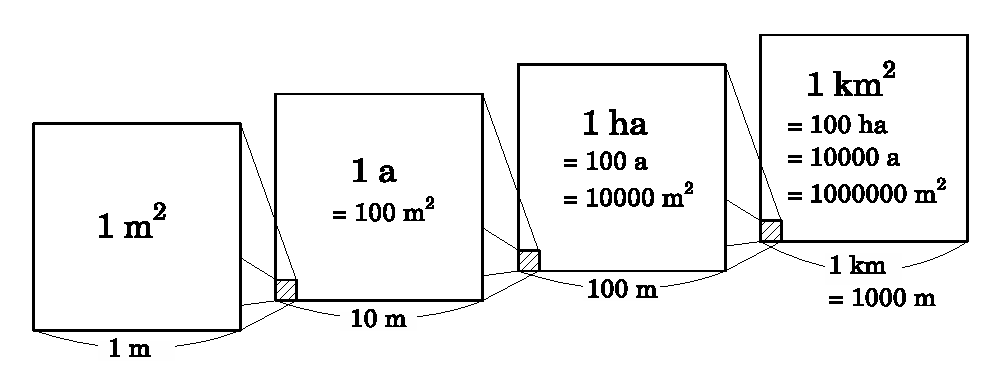
\includegraphics[width=8.2cm]{area_km2_ha.eps}
    \caption{いろいろな大きさの正方形の面積}\label{fig:area_km2_ha}
\end{figure}

\begin{q}\label{q:alg_unit1} 以下の量を書き換えよ:
\begin{edaenumerate}<2>
\item 1~mをkmで。
\item 1~kmをmで。
\item 1~cmをmで。

\item 1~m$^2$をkm$^2$で。
\item 1~km$^2$をm$^2$で。
\item 1~cm$^2$をm$^2$で。

\item 1~m$^3$をkm$^3$で。
\item 1~km$^3$をm$^3$で。
\item 1~cm$^3$をm$^3$で。

\item 1~dm$^3$をm$^3$で。
\item 1~dLをm$^3$で。
\item 1~$\mu$mをmで。

\item 1~$\mu$mをnmで。
\item 1~mgをkgで。
\item 1~km$^2$をhaで。
\end{edaenumerate}
\end{q}

{\small 注: dLは, 小学校以外ではほとんど使われない。これは, 1 dLの
立方体の1辺が, $(0.0001\,\text{m}^3)^{1/3}=0.0464\cdots$~mという
中途半端な数値になるからだろう。}

\begin{q}\label{q:alg_unit2} 以下の量を書き換えよ(導出過程も書け):
\begin{edaenumerate}
\item 0.009 km$^2$をm$^2$で。
\item 0.00003 km$^3$をm$^3$で。
\end{edaenumerate}
\end{q}

\begin{q}\label{q:alg_unit3} 以下の各小問内で, 挙げられた2つの単位が
互いに等しいことを示せ:
\begin{edaenumerate}
\item mLとcm$^3$。
\item Lとdm$^3$。
\item kLとm$^3$。
\item GtとPg。
\end{edaenumerate}
\end{q}

{\small 注: もともとLは「質量1~kgの水の体積」と定義されていたが, 
水は温度や圧力によって体積を微妙に変えるので, 体積の単位として
ふさわしくない。現在は, Lは10$^{-3}$~m$^3$のことであると
再定義され, なおかつ, 古い定義(水1~kgの体積)と紛らわしい
ので, Lはなるべく使わず, かわりにdm$^3$ (立方デシメートル)
と言おう, というのがSI単位系の立場である。\\}

SI単位系では他にもいろいろな約束が決まっている。特に, 
以下を覚えておこう:
\begin{itemize}
\item 変数や定数を表すアルファベットは斜体表記せよ。\\
例: $x=5$はOK, x$=5$はダメ。
\item 特定の関数を表すアルファベットは立体表記せよ。\\
例: $\sin x$はOK, $sin\,x$はダメ。
\item 単位を表すアルファベットは立体表記せよ。\\
例: 面積を表す$5\,\,\text{m}^2$はOK, $5\,\,m^2$はダメ。
\item 数値と単位の間には半角スペースをあけよ。\\
例: $5\,\,\text{m}^2$はOK, $5\text{m}^2$はダメ。
\item 組み立て単位は, 単位どうしの間に半角スペースをあけよ。\\
例: 速度を表す2 m~s$^{-1}$はOK, 2 ms$^{-1}$はダメ。
\item 接頭辞と単位の間にはスペースをあけるな。\\
例: 3~kgはOK, 3 k gはダメ。
\end{itemize}
最後の2つは特に大切。そのおかげで, 1~ms (1ミリ秒)
と1~m~s (1メートル秒)が区別できる。

科学技術文書のほとんどはこういう表記を使っている。
日本ではJIS規格になっている\footnote{しかし, なぜか日本の小中学校の検定教科書では, 
単位が斜体で書かれている。高校の教科書では立体になっているのだが...}。
本書も極力, この表記法に従う(一部, コンピュータソフトの仕様上の制限の為にうまく
できなかったところもあるが)。

レポートや卒業論文ではこれらに注意しよう。
ただし, 手書きでは無理に守らなくてもよい。
立体と斜字体の書き分けや, 「半角スペース」
は手書きでは無理だし。そこで, 手書きの時は, 
単位を括弧[ ]の中に入れて書いたりする。
例えば, 5.3~m/sを, 5.3~[m/s]と書くのだ。\\



\section{単位の換算}
\begin{exmpl}\label{exmpl:7.5km/h} 7.5 km~h$^{-1}$という量を, m~s$^{-1}$という単位に換算してみよう。
\begin{eqnarray}
7.5\,\,\text{km h}^{-1}&=&7.5\,\,\frac{\text{km}}{\text{h}}=7.5\,\,\frac{1000\text{ m}}{3600\text{ s}}\nonumber\\
&=&7.5\times\frac{1000}{3600}\text{ m s}^{-1}=2.08\cdots\text{ m s}^{-1}\nonumber\\
&\fallingdotseq&2.1\text{ m s}^{-1}
\end{eqnarray}
最後に2.08の8を四捨五入した。有効数字を考えたからである。7.5の有効数字が2桁であると判断されたので, 結果も有効数字2桁にした。\end{exmpl}

\begin{exmpl}\label{exmpl:2.0g/s} 2.0 g/sという量を, kg/hという単位で換算してみよう。
\begin{eqnarray}
&&2.0\,\,\text{g/s}=2.0\,\,\frac{\text{g}}{\text{s}}=2.0\,\,\frac{10^{-3}\text{ kg}}{(1/3600)\text{ h}}
=2.0\times\frac{3600}{1000}\text{ kg/h}\nonumber\\
&&=2.0\times3.6\text{ kg/h}=7.2\text{ kg/h}
\end{eqnarray}
(例おわり)\end{exmpl}\mv

これらの例でわかるように, 単位の換算は機械的にできる。
組み立て単位を構成する各単位(h, s, km, m, kg, gなど)を, 
それぞれ別の単位に換算し, そこで出てきた係数を計算すればよいのだ。\mv

上の例のやり方がよくわからない人には, かわりに, 
次の方法を勧める。例\ref{exmpl:7.5km/h}は,
\begin{eqnarray}
7.5\,\,\text{km h}^{-1}&=&7.5\,\,\frac{\text{km}}{\text{h}}\label{eq:unit_conv_mult1_02}\\
&=&7.5\,\,\frac{\text{km}}{\text{h}}\,\,\frac{1000\text{ m}}{\text{km}}\,\,\frac{\text{h}}{3600\text{ s}}\label{eq:unit_conv_mult1_04}\\
&=&7.5\,\,\frac{10\teisei{00}}{36\teisei{00}}\,\,\frac{\teisei{\text{km}}}{\teisei{\text{h}}}\,\,\frac{\text{ m}}{\teisei{\text{km}}}\,\,\frac{\teisei{\text{h}}}{\text{ s}}\label{eq:unit_conv_mult1_06}\\
&=&\frac{75}{36}\,\frac{\text{ m}}{\text{ s}}=2.08\cdots\text{ m s}^{-1}\\
&\fallingdotseq&2.1\text{ m s}^{-1}\label{eq:unit_conv_mult1_08}
\end{eqnarray}
ここで, \eref{eq:unit_conv_mult1_02}から\eref{eq:unit_conv_mult1_04}に行く時に, 
\begin{eqnarray}
\frac{1000\text{ m}}{\text{km}}\quad\text{と}\quad\quad\frac{\text{h}}{3600\text{ s}}\label{eq:unit_conv_times1}
\end{eqnarray}
をかけているが, これらは両方とも1だ。なぜなら, 1000~m=1~kmであり, 
両辺をkmで割ると, (1000~m)/km=1となる。同様にしてh/(3600~s)=1も言える。
これらの1は単位を持たぬ量(無次元量)だ。1を掛けても, 掛けられた量は何も
変化しない。そこで, \eref{eq:unit_conv_times1}のような, 「1と等しい量」
を自由にどんどん掛けて, 消し去りたい単位を約分していくのだ。

\begin{freqmiss}{\small\textgt{7.5~km/h = 27000000~m/sという, 
とんでもない間違いをする}... これは, 3600で割らねばならぬところを, 
3600を掛けてしまったミスです。この手のミスは, 計算過程で単位を埋め込まずに, 
数値だけで処理すると発生しがちです。でも, そもそも, 7.5~km/hは
徒歩(小走り)や自転車くらいの速さなので, 秒速2700万メートル
なんかになるわけがありません。\textgt{物理量を実際の現象と結びつけて
感覚的に把握する}習慣をつけましょう。}\end{freqmiss}

\begin{q}\label{q:unit_conv_mult1} 上で述べた, 1を掛けていく方法
で, 例\ref{exmpl:2.0g/s}の単位換算をやり直せ。\end{q}

\begin{q}\label{q:alg_unit4} 以下の量を書き換えよ。上で示した2つの方法の
どちらを使っても構わない。ただし, 導出過程も書くこと。電卓を使ってもOK。
\begin{enumerate}
\item 340~m/sをkm/hで。(音速)
\item $3.00\times10^8$~m/sをkm/hで。(光速)
\item 1.0~g/cm$^3$をkg/Lで。(水の密度)
\item 1.0~g/cm$^3$をt/m$^3$で。(水の密度)
\item 1.3~g/Lをkg/m$^3$で。(空気の密度)
\item 0.05~kg/hをg/sで。
\end{enumerate}
\end{q}
\mv

上のような問題では, 結果を科学の法則や現象に整合しているか
チェックしよう。例えば(1)は音速だが, 音速といえば飛行機だ。
音速を超えると急に抵抗が大きくなって燃料をたくさん喰う
ので, 多くの旅客機は音速より少し遅く飛ぶ。従って, 
(1)は, 旅客機が1時間で飛べる距離とだいたい同じはず。
飛行機に乗ったことのある人は, 旅客機は1時間で東京から九州とか
北海道の手前くらいまで飛ぶと知っているだろう。

\begin{q}\label{q:scale} 以下の量とおおよそ桁が合うような, 
具体的な現象や事物(数値を使わずに表現できるもの)
を述べよ。例: 1~ha ... 日本の平均的な農家1戸の耕作面積, 
1~L ... コンビニで売ってる中くらいの大きさのお茶のPETボトル。
\begin{edaenumerate}<3>
\item 1~mL
\item 1~m$^3$
\item 1~mg
\item 1~g
\item 1~kg
\item 1~t
\item 1~$\mu$m
\item 10000~km
\item 100000~km$^2$
\end{edaenumerate}
\end{q}
\mv

ところで, 物質の量は, 多くの場合は質量で表すが(「質量保存の法則」
があるから!), 体積で表すこともある。例えば3~tの水を
「3~m$^3$の水」と言ったりもする。すなわち, 
\begin{eqnarray}
3 \text{ t}\text{の水}=3 \text{ m}^3\text{の水}\label{eq:water_m3eq_t}
\end{eqnarray}
と言ってよい。だからといって, 
\begin{eqnarray}
\text{t}=\text{m}^3\quad\quad\text{(これは間違い!)}\label{eq:m3eq_t}
\end{eqnarray}
と言ってはダメ。そもそもtは質量, m$^3$は体積なのだから, これら
が同じなわけがない。もし\eref{eq:m3eq_t}が正しければ, 1~tの空気の体積も
1~m$^3$になってしまう(本当は約770~m$^3$)。\eref{eq:water_m3eq_t}が成り立つのは, 
水の密度がほぼ一定だからだ。密度が一定であれば, 質量と体積は
比例するから, どちらを使っても実用上は構わない。しかし, そこには
「密度」という重要な量が背後にあることを忘れてはダメ。


\begin{q}\label{q:rice_weight_vol} コメの量も, 重さ(質量)で
表したり, 体積で表したりする。コメのバルク密度を調べよ。(バルク
密度とは, たくさんの米粒を容器に入れた時のように隙間も含んだ
状態での密度)。それを元に, 10 kgのコメの体積を求めよ。\end{q}
%まだ答を作ってない!
\mv

\begin{faq}{\small\textgt{\eref{eq:water_m3eq_t}で両辺の「の水」を
約分すれば3~m$^3$=3~tになるから, \eref{eq:m3eq_t}も正しいのでは?}
 ... ダメ。約分は「何か×何か」の形の量について片方の「何か」
を割って消すこと。「3~m$^3$の水」は, 「3× 1~m$^3$の水」です。
1~m$^3$の水が3個分, という意味。でも君の考えでは, 
「3~m$^3$×水」と解釈して「水」だけを約分しています。これは無茶です。}
\end{faq}
\mv


\section{力の単位}

理系はどんな分野でも, 力やエネルギーの概念(中学理科の1分野)が
基礎だ。さらにその基礎は, 
\begin{itembox}{運動の法則(ニュートンの運動方程式)}
質量$m$の物体が力${\bf F}$を受けたとき, 物体の速度は変化する。
その変化率, つまり加速度(速度の変化を時間で割ったもの)を${\bf a}$とすると,
\begin{eqnarray}{\bf F}=m{\bf a}\label{eq:Newton_eqmotion}\end{eqnarray}
\end{itembox}
である。これは中学理科や高校の物理基礎で学んだ! これは全ての科学における
最も大切な常識のひとつである。この式を「知らない」という人がいるが, 
それは「細胞」とか「イオン」を知らないというくらいヤバい。

この式は, 本書の他の多くの数式とは根本的に性格が異なる。本書の多くの
数式は「定義」や「公理」か, それらをもとに導出される「定理」か, それらを
用いた計算式だ。ところが, この式はそのいずれでもない。
数式の格好をしているが, 自然の摂理を表す\underline{「基本原理」}
(基本法則ともいう)である。
そしてこの式の根拠は, 公理でも論理でもなく, 実験事実である。

ちなみに\eref{eq:Newton_eqmotion}で, ${\bf F}$はforce (力), 
$m$はmass (質量), ${\bf a}$はacceleration (加速度)
のそれぞれ頭文字から取られている。このように, 科学の
数式で出てくる記号は, その量の頭文字から取られることが多い。

\begin{freqmiss}{\small\textgt{「運動方程式を書け」という問に対して「${\bf F}=m{\bf a}$」とだけ答える}
 ... ${\bf F}, m, {\bf a}$のそれぞれが何を意味するかも, 書き添えなければなりません。}
\end{freqmiss}

\begin{faq}{\small\textgt{${\bf F}$と${\bf a}$の活字の形がなんか他と違うっぽいんですが...}
 ... よく気づきましたね。これは\pref{sect:vector_digest}あたりで学んだ「ベクトル」です。
力には大きさだけでなく向きもあるから, ベクトルです。加速度もそうです。だから, ベクトルの
書き方(太字)で書いているのです。}\end{faq}
\mv

さて, SI単位系では力の単位はN (ニュートン\footnote{いわずと知れた
イギリスの物理学者の名前。運動の法則と万有引力の法則
を発見した, 科学界のスーパースター。})である。\eref{eq:Newton_eqmotion}
において, ${\bf F}$をその単位であるNに置き換え, $m$をその単位であるkgで
置き換え, ${\bf a}$をその単位であるm s$^{-2}$で置き換えると, 
\begin{eqnarray}
\text{N}=\text{kg m~s}^{-2}\label{ed:def_N}
\end{eqnarray}
となる。これがNという単位の定義である。この式を忘れても, ${\bf F}=m{\bf a}$を覚えて
いれば, 上記のように考えればすぐに思い出せるだろう。

\begin{faq}{\small\textgt{加速度の単位がm s$^{-2}$, というのがわかりません。}
 ... 加速度は, ざっくりいうと, 速度の変化を時間で割ったものです(正確な定義は
後の章で説明します)。速度の単位はm s$^{-1}$ですから, 速度の変化(つまり, ある時刻の
速度ひく別の時刻の速度)の単位もm s$^{-1}$です。それを時間(単位はs)で割るのだから, 
最終的に単位はm s$^{-2}$になります。}\end{faq}

ところで, 「重さ」と「質量」を混同している人がいる。これはヤバイ。 重さは
その物体に働く重力のこと。重力は力の一種だ。だから重さは力の単位(SI単位系ではN)で表すのが, 科学的には正しい。
重さは場所によって変わる。同じ物体でも, 月面上での重さは地上での重さの
約1/6になるし, 国際宇宙ステーションの中(いわゆる無重力空間)
では重さは0~Nだ。

一方, 質量は, 力とは別の量だ。地球上だろうが月面上だろうが
無重力空間中だろうが, 同じ物体の質量は不変である。地球上で
1~kgの物体は, 月や国際宇宙ステーションに持って行っても1~kgなのだ。

えっ!? どういうこと!? と思う人は, ここから先を
慎重に読んでしっかり考え, 必ず理解しよう。まず質量
とは何だろう? それは\eref{eq:Newton_eqmotion}が教えてくれる。
\eref{eq:Newton_eqmotion}によると, 一定の力${\bf F}$を物体に
かけたとき, 質量$m$が大きい物ほど加速度${\bf a}$は小さいし, 
$m$が小さいほど${\bf a}$は大きいことがわかる。つまり質量$m$は
物体の「速度の変えにくさ」(加速度は速度が単位時間あたりに
どれだけ変化するか, という量であることに注意!), 
つまり「動かしにくさ」を表す。それは無重力空間でも変わらない。
国際宇宙ステーションの中に1~kgの物体と10~kgの物体の2つを
ぷかぷかと浮かせて, それらを同じ力で同じ時間だけ押すと, 
1~kgの物体の方がずっと速く飛んでいくだろう。

「重さ」の本質は, \eref{eq:Newton_eqmotion}とは別の
重要な物理法則が教えてくれる。それは, 「どんな物体どうしにも, 
互いに引き合う力が生じ, その大きさは, 2つの物体の質量の積に比例し, 
距離の2乗に反比例する」という法則だ。そのような力のことを重力と言うのだ。
地表で物体が地球から受ける重力は, その物体の質量と地球の質量の積に
比例し, 地球半径の2乗に反比例する。地球質量と地球半径はほぼ一定
なので, 「地表限定」の条件下では, 重力(つまり重さ)は, 物体の
質量だけで決まる。1~kgの物体の重さ(重力)は地表上のどこでも
約9.8~Nでほとんど変わらないので, 「1~kgの物体の地上での重さ」
を力の単位としてもよいだろう。そう定義された力の単位のことを, 
kgfという(kg重ともいう)。正確な定義では, 
\begin{eqnarray}
1 \text{ kgf}:=9.80665\text{ N}
\end{eqnarray}
である。実際, 土木や建築等の工学では力をkgfで表すことが多い。
しかし, kgfはSI単位系の単位ではないので, 科学ではkgfを使うことは
避ける方がよい。

ところで, 世の中では往々にしてkgfのfが略されて「kg」と言われて
しまう。一方, 日常生活では, 質量と重さは頻繁に混同され, 「A君の
体重は60~kg」というような表現が多い。でも体重とは「体の重さ」
なので, 正しくは「A君の体重は60~kgf」もしくは「A君の質量は60~kg」
とすべきである。

日常生活では体重と質量を混同したり, kgfをkgと誤記しても困らないので, 
そんなにこだわる必要は無い。しかし科学の世界では, 明確に区別
せねばならない。\mv

\begin{faq}{\small\textgt{中学校で, 「100 g = 1 N 」と
習ったのですが...} ... それは間違い。100~gは質量, 1~Nは
力なので, 両者は互いに次元が異なるから, 等号で結ぶことは
できません。ただ, 「質量100~gの物体\textgt{にかかる重力の大きさ}
は約1~Nである(正確には0.98~N)」というのは正しいし, 私が
チェックした中学校の教科書にはそのように載っていました。
「100 g = 1 N 」のような乱暴な間違いが載っているのは, 
塾のプリントや参考書のようです。\\
\textgt{それのどこがダメなのか, いまいちわかりません...} ... 
例えで説明しましょう。1~Lの水の質量は(ほぼ)1~kgです。
だからといって、 1~L=1~kgと言ってはダメでしょう。
左辺は体積, 右辺は質量なのだから。それと同じこと。}\end{faq}

\begin{q}\label{q:kgf} 60~kgfは何Nか? 有効数字2桁で。\end{q}
\hv


\section{エネルギーと圧力の単位}\label{sect:energy_pressure}

次に, 仕事とエネルギーの定義を確認しよう。これらも中学校理科であり, 
知らなきゃヤバイことである:
\begin{itembox}{仕事とエネルギーの定義} 
物体に力をかけて移動させるとき, 力と, その力の方向に動いた
距離との積を, 「仕事」\index{しごと@仕事}という。仕事と等価な量(仕事に形を
変えることができる量)のことを「エネルギー」\index{えねるぎー@エネルギー}という。
\end{itembox}

ざっくり言えば, 「仕事=力×距離」である。SI単位系では, 仕事の単位は
J (ジュール\footnote{イギリスの物理学者の名前。電気回路で
出る熱に関する「ジュールの法則」を発見した人。})だ。
「仕事=力×距離」で, 「仕事」をその単位であるJで置き換え, 「力」を
その単位であるNで置き換え, 「距離」をその単位であるmで置き換えれば, 
\begin{eqnarray}
\text{J}=\text{N m}\label{ed:def_J}
\end{eqnarray}
となる(定義)。\eref{ed:def_J}を忘れても, 「仕事=力×距離」
を覚えていれば, 思い出せるだろう。\\

エネルギーは仕事と等価な量なので, エネルギーのSI単位は仕事と同じJである。\\

また, 中学校理科で学んだように, 面に一様に力がかかるとき, 
その力を面積で割ったものを圧力という。ざっくり言えば, 
「圧力=力/面積」だ。SI単位系では, 圧力の単位はPa (パスカル
\footnote{フランスの哲学者かつ物理学者の名前。「人間は考える葦である」
との言葉を残した人。})である。
「圧力=力/面積」で, 「圧力」をその単位であるPaで置き換え, 「力」を
その単位であるNで置き換え, 「面積」をその単位であるm$^2$で置き換えれば, 
次式になる:
\begin{eqnarray}
\text{Pa}=\text{N/m}^2=\text{N m}^{-2}\label{ed:def_Pa}
\end{eqnarray}
これがPaの定義である。\eref{ed:def_Pa}を忘れても, 「圧力=力/面積」
を覚えていれば, 思い出せるだろう。\\

また, 中学校理科で学んだように, ある時間内になされた仕事や, 出入りした熱や, 
エネルギーの増減量を, その時間で割ったものを, 仕事率又は熱効率という。
ざっくり言えば, 「仕事率=仕事/時間」である。SI単位系では, 
仕事率の単位はW (ワット\footnote{イギリスの発明家の名前。
蒸気機関を開発して, 産業革命に貢献した人。})である。
「仕事率=仕事/時間」において, 「仕事率」をその単位であるWで置き換え, 
「仕事」をその単位であるJで置き換え, 「時間」をその単位であるsで置き換えれば, 
\begin{eqnarray}
\text{W}=\text{J/s}=\text{J s}^{-1}\label{ed:def_W}
\end{eqnarray}
となる。これがWの定義である。\eref{ed:def_W}を忘れても, 「仕事率=仕事/時間」
を覚えていれば, 思い出せるだろう。

\begin{freqmiss}{\small\textgt{WとJを混同する} ... 
JとWは明確に異なる単位です。W=J/s, J=W sです。}\end{freqmiss}

ところで, 電気的なエネルギーや電気がする仕事を「電力量」\index{でんりょくりょう@電力量}という。また, 
電気がする仕事の仕事率を「電力」\index{でんりょく@電力}という。

\begin{freqmiss}{\small\textgt{Wは電気専用の単位だ
と思っている} ... 
Wは仕事率の単位なので, 電力以外の仕事率にも使われます。
おそらくこういう誤解をする人は, 中学校で習った
W=A$\times$V (Aはアンペア, Vはボルト)に引きずられて
いるのでしょう。それは間違いではないけど, Wの定義では
ありません。}\end{freqmiss}

\begin{q}\label{q:state_F=ma_etc} 
\begin{enumerate}
\item ニュートンの運動方程式を書け。
\item 仕事の定義を書け。
\item エネルギーの定義を書け。
\item 圧力の定義を書け。
\item 仕事率の定義を書け。
\end{enumerate}\end{q}

\begin{q}\label{q:unit_NJPaW_matome7} 以下の問に答えよ。
導出過程も書くこと。
\begin{enumerate}
\item 質量2$\,\,$kgの物体を加速度3 m~s$^{-2}$で加速するのに必要な力は?
\item ある物体を2 Nの力で4 mだけ移動させるのに必要なエネルギーは?
\item 2$\,$m$^2$の平面に10$\,$Nの力がかかっている状態の圧力は?
\item 100$\,\,$Wの電球が, 2秒間に消費する電力量は?
\end{enumerate}
\end{q}

\begin{q}\label{q:unit_NJPaW_relation} 以下を示せ:
\begin{edaenumerate}
\item N = J / m
\item Pa = J~m$^{-3}$
\item J = Pa~m$^3$
\item J/Pa = m$^3$
\item W = N~m~s$^{-1}$
\item J = W~s
\end{edaenumerate}
\end{q}
\mv

\begin{q}\label{q:unit_NJPaW_matome1} J, Pa, Wを, 
それぞれSI基本単位(kg, m, s)の組み合わせで表わせ。\end{q}

\begin{q}\label{q:kWh2J_hPa2Pa} 以下の量を書き換えよ:
\begin{edaenumerate}
\item 1~kW hをJで。
\item 1~hPaをPaで。
\end{edaenumerate}
\end{q}
\mv

ところで, 圧力の単位にatm (気圧)というのがある。定義は
$1\text{ atm} :=1013.25\text{ hPa}$である
(hPaのhを忘れる人が多い)。atmはatmosphereの略である。
1~atmのことを1~気圧ともいう。

\begin{q}\label{q:unit_atm_Pa_conversion} 以下の問に答えよ。電卓を使ってもよい。
\begin{enumerate}
\item 1~atmをPaで表わせ。
\item 1~atmをkPaで表わせ。
\item 1~Paをatmで表わせ。
\item ある巨大な台風(実際にあった!)の中心付近での地表での気圧は895~hPaだった。
この圧力をatmで表わせ。
\end{enumerate}
\end{q}

高校の化学や物理で学んだように, 理想気体の圧力$P$, 体積$V$, 
モル数$n$, 絶対温度$T$, 気体定数\index{きたいていすう@気体定数}$R$の間には, 
$PV=nRT$という関係が成り立つ(理想気体の状態方程式)。また, $R=8.3145~\text{J~mol}^{-1}\text{K}^{-1}$
である。

\begin{q}\label{q:PVnRT} 1.0000~molの理想気体が, 温度273.15 K, 
1013.25 hPaにあるときの体積を計算し, Lで表せ。電卓使用可。\end{q}

\begin{q}\label{q:gas_const_conversion} 気体定数$R=8.3145$~J~mol$^{-1}$~K$^{-1}$
の値を, atm~L~mol$^{-1}$~K$^{-1}$という単位で書き換えよ。
電卓使用可。途中経過も書け。ヒント: J=Pa~m$^3$。\end{q}

ところでエネルギーの単位にカロリー(cal)というのもある。
定義は, $1\text{~cal}:=4.184\text{~J}$である(記憶せよ)。もともと, 
1~calは「質量1~gの水の温度を1$^\circ$C上げるのに必要
な熱量」と定義されていたのだが, それは条件次第で
微妙に異なるので, 今は上のようにJとの関係で定義されている。

\begin{q}\label{q:water_specific_heat} 常温・液体の
水の比熱を, J kg$^{-1}$ K$^{-1}$という単位で表わせ。
\end{q}

\begin{q}\label{q:cal_J} 以下の問に答えよ:
\begin{enumerate}
\item 成人ひとりが1日に食物から摂取するエネルギーは約2500~kcal
である。この量をJで書き換えよ。
\item 上記のエネルギーを全部熱にすると, 体積0.5~m$^3$の水
(風呂桶1杯くらい!)の温度を何Kだけ上げることができるか?
\item 上記のエネルギーを全部仕事にすると, 質量10~kgの
物体を地上からどのくらいの高さまで持ち上げることができるか?
\end{enumerate}
\end{q}
\mv

\begin{comment}
\section{物理量を表す記号}

\eref{eq:Newton_eqmotion}で$F=ma$が出てきたとき, 
$F$は力, $m$は質量, $a$は加速度だった。でも, 例えば
力を$A$, 質量を$B$, 加速度を$C$とすれば, 
\eref{eq:Newton_eqmotion}は$A=BC$と書いても構わない。
このように, 原則的には, 物理量は, 各自が記号を自由に定義して使ってよいのだ。

でも, 規則ではないが「この物理量はこの記号を使うのが普通だよね」
という慣習というか常識というか空気がある。いわば, 犬の名前はポチ, 
猫の名前はタマ, みたいなものだ。その代表的なものを以下に示す:

\begin{table}[!htb]\caption{物理量の慣習的な記号と単位}
\begin{center}
\begin{tabular}{ccc}\hline
物理量 & 記号 (由来) & 単位 \\\hline
質量 & $m$ (mass) & kg \\
時刻 & $t$ (time) & s \\
長さ, 位置 & $l$ (length), $x$等 & m \\
面積 & $a$, $A$ (area), $S$ (surface) & m$^2$ \\
体積 & $V$ (volume) & m$^3$ \\
速度 & $v$ (velocity) & m s$^{-1}$ \\
加速度 & $a$ (acceleration) & m s$^{-2}$ \\
力 & $F$ (force) & N \\
仕事 & $w$, $W$ (work) & J \\
仕事率 & $P$ (power) & W \\
圧力 & $p$, $P$ (pressure) & Pa \\
分子数 & $n$, $N$ (number) & 個, 又はmol \\
熱量 & $q$, $Q$ & J \\
エネルギー & $E$ (energy), $U$, $K$, $T$& J \\
温度 & $T$ (temperature) & K \\\hline
\end{tabular}
\end{center}
\end{table}
これらは覚えなくてもよいが, 慣れるのが望ましい。
紛らわしいのが, 別々の物理量の記号と単位に同じようなアルファベット
が現れる場合。例えば$m$は質量を表す一方, mは長さの単位である。
$W$は仕事を表す一方, Wは仕事率の単位である。しかし
こういうのは, 物理量は斜字体, 単位は立体, という, 
字体の用法で区別できる。だから字体は大事なのだ。

また, 同じ記号が, 違う物理量に出てくる(かぶる)ことも
ある。例えば$P$は, ときに仕事率, ときに圧力を表す。だから, 
物理量の記号は, たとえ「それが常識」でも, 毎回その場その場で
定義し直さねばならない。\\
\end{comment}

\section{dimension check}
ここで, ひとつ, 便利な道具を紹介しよう。

\begin{exmpl}
高校の物理基礎で学んだように, 質量$m$の物体が速さ$v$で移動しているとき, 
その物体の持つ運動エネルギー$K$を次式で定義する:
\begin{eqnarray}
K:=\frac{1}{2}m\,v^2\label{eq:def_kinenergy}
\end{eqnarray}
この両辺の単位をSI単位で考えよう。まず1/2は無次元量なので
単位なし。$m$の単位はkg, $v^2$の単位は(m s$^{-1}$)$^2$=m$^2$~s$^{-2}$。
従って, 右辺の単位はkg m$^2$~s$^{-2}$。これはJである
(問\ref{q:unit_NJPaW_matome1}参照)。一方, 左辺の$K$は
「エネルギー」と呼ばれる以上, SI単位ではJで表現できる
はずである。従って, この両辺は, 同じ単位で揃えることが
できる(次元が同じ!)。(例おわり)\end{exmpl}

このように, ある式について, 両辺が同じ単位を持てるかを調べること
(すなわち両辺で次元が一致しているか調べること)を, 
dimension check\index{dimension check}という。
等式の両辺は, 互いに同じ物理量を表すのだから, 
同じ単位で表すことができる(次元が一致している)はず。
ところが, 何かミスをすると(例えば\eref{eq:def_kinenergy}
の$v^2$の2乗を忘れたり), 左辺と右辺で単位は一致
しなくなることが多いので, これは, その式が正しく
できているかどうかの検算に使える。

実は, これに似た考え方を, 既に例\ref{exmpl:niku600yen}や
例\ref{exmpl:mihaji}で紹介した。つまり, 単位を式に埋め込んで
計算すれば, 結果的にdimension checkにもなるのだ。\mv

\begin{q}\label{q:unit_dimcheck} \eref{eq:rect_area00_NG}
のような書き方が不合理であることを, dimension checkの観点で
説明せよ。\end{q}

\begin{q}\label{q:potentialE_dim} 高校の物理基礎で学んだように, 
地表付近で, 質量$m$の物体が高さ$h$にあるとき, その物体の持つ
位置エネルギー$U$は次式で表される\footnote{これは位置エネルギー
の定義ではない。位置エネルギーは, これとは別の式で定義され, そこから
この式が演繹される。また, 大学では位置エネルギーを
「ポテンシャルエネルギー」と呼ぶ。}。
\begin{eqnarray}
U=mgh
\end{eqnarray}
$g$は重力加速度と呼ばれる定数で, $g\fallingdotseq9.8$~m~s$^{-2}$である。
この式をdimension checkせよ。
\end{q}

\begin{q}\label{q:sphere_SV_dimcheck} 半径$r$の球の
表面積$S$と体積$V$はそれぞれ
\begin{eqnarray}
&&S=4\pi r^2\label{eq:ball_surface}\\
&&V=\frac{4}{3}\pi r^3\label{eq:ball_volume}
\end{eqnarray}
である。ところが, 君の友人A君は, この公式を逆に
覚えている($V=4\pi r^2$, $S=4\pi r^3/3$と覚えている)。
dimension checkを使って, A君に間違いを
教えてあげるには, どう言えばよいか?
\footnote{$S$はsurfaceの頭文字, $V$はvolumeの頭文字, 
そして$r$はradiusの頭文字に由来する。このように, 
量を表す記号(アルファベット)は, その英単語に
由来することが多い。それも公式を覚えたり思い出したり
するときの手がかりになる。}\end{q}

%\begin{q}\label{q:dim_fric_coeff} ある物体が別の物体と接触して, 互いに摩擦を及ぼしながら
%動いているとき, 両者にかかる摩擦力を$F_{\text{m}}$とすると, それは
%接触面を介して両者が互いに垂直に押し合う力$N$に比例する, ということが
%わかっている(クーロンの摩擦法則の一部)。すなわち, 
%\begin{eqnarray}F_{\text{m}}=\mu'N\label{eq:law_friction_m}\end{eqnarray}
%と書ける。このときの比例係数$\mu'$のことを「動摩擦係数」と呼ぶ。
%動摩擦係数の次元は無次元であることを示せ。\end{q}
\hv


\section{例外!}
ここで, 少しやっかいな話。「物理量は数値と単位の積」
と述べたが, そうではない場合が存在するのだ。

もし物理量が「数値と単位の積」なら, その「数値」が0の
ときにはその物理量は0である。例えば, 0 mは長さが0 (無い)
ということである。

すると, 「数値が0でも物理量が0にならない場合」は, 
「数値と単位の積」ではない, ということになる(これは上
で述べたことの対偶である。対偶がわからない人は, 
索引で調べよ)。そして, 実際にそのような場合があるのだ!

\begin{exmpl} 温度はそもそも, 分子の平均運動エネルギー
に比例するような物理量であり, その単位としてK (ケルビン)
が使われる。当然, 分子の平均運動エネルギーが0
のときの温度は0 Kである。ところが, 温度を摂氏で表すと, 
$0\ {}^\circ\mathrm{C}$のときは273~Kであり, 0~Kではない。
\end{exmpl}

\begin{exmpl} pHは, 水溶液の中の
水素イオンの濃度\index{すいそいおんのうど@水素イオン濃度}[H$^+$]
の指標であり, 次式で定義される:
\begin{eqnarray}
\text{pH}:=-\log_{10}\frac{\text{[H}^+\text{]}}{\text{mol~L}^{-1}}\label{eq:define_pH}
\end{eqnarray}
%[H$^+$]が$10^{-7}\,\,$mol L$^{-1}$である水溶液のpHは7であり, 
%[H$^+$]10倍になるたびにpHは1下がる, と約束する。例えば, 
%pHが5の水溶液は[H$^+$]=$10^{-5}\,\,$mol~L$^{-1}$である。
\end{exmpl}

\begin{q}\label{q:pH2density} 次式を示せ:
\begin{eqnarray}
\text{[H}^+\text{]}=10^{-\text{pH}}\text{ mol~L}^{-1}\label{eq:pH2density}
\end{eqnarray}
\end{q}

\begin{q}\label{q:pH0} pHが$-1$の水溶液の水素イオン濃度は?\end{q}

\begin{q}\label{q:exp_pH} 
\begin{enumerate}
\item 水素イオン濃度が0.005 mol~L$^{-1}$のときpHは?
\item pH=5.6のとき, 水素イオン濃度は中性(pH=7)のときの何倍か? 
\item pH=5.0の塩酸と, pH=3.0の塩酸を, 等量, 混ぜ合わせたら, 
pHはどのくらいになるか? ただし塩酸はすべて解離するものとする。
\end{enumerate}\end{q}

%\begin{exmpl} 君が受験でお世話になった「偏差値」は, 個々の学生
%の成績が, 受験生全体の中でどのくらいかを表す(その定義は本書の後半
%で学ぶ)。ところが, 得点が0点でも偏差値30とか40ということはよくある。
%(例おわり)\end{exmpl}

ここで示した2つの例は, 「数値と単位の積」ではない。つまり, 
$\ {}^\circ\mathrm{C}$やpHという単位は, 普通じゃない, 
変な単位である。こういう単位は, 単位同士の掛け算, 割り算, 約分
はできないし, それを利用した単位換算法も使えないし, 
\eref{eq:L/cm=15}のような表現もできないし, dimension checkも使えない。
なので, こういう単位のからむ計算や変換は, ケースバイケースで慎重に
対応しなければならない。

\begin{faq}{\small\textgt{「ケースバイケースで慎重に対応」って, 
具体的にはどういうことですか?}... いちばん簡単なのは, 単位換算や
他の量と一緒に計算する時にはそういう量を「数値と単位の積」
に書き換えてしまうことです。$\ {}^\circ\mathrm{C}$は
Kに, pHはmol L$^{-1}$に書き換えてしまうのです。}\end{faq}


%同様の事情は, 地震の規模を表すマグニチュード\index{まぐにちゅーど@マグニチュード}
%という指標や, 音の大きさを表すデシベル\index{でしべる@デシベル}という指標にもある。
%これらの特殊な単位には, 「対数」という考え方が背景にある(対数については第\ref{chapt_exp_log}章で学ぶ)。\\
%\hv

% 摂氏とK。
% 0度C=273Kの両辺を2倍したら, 0度C=546K。何がおかしい?
% 度CとKは比例しない。
% 同じことが摂氏と華氏でも起きる。
% 度Cは「単位」とは言えない。
% 例: 100点満点のテスト。40点=偏差値50。両辺を2倍したら, 80点=偏差値100? 何かおかしい。
% 得点と偏差値は比例しない。
% 同じ対象でも, 表現の仕方によって, 数学的な性質が大きく異なる。そういう場合はイコールで結んではいけない(おかしなことになる)。
\mv


\section*{演習問題}

\begin{exq}\label{q:degC_K} $0\ {}^\circ\mathrm{C}$は273 Kである。
つまり, 
\begin{eqnarray}
0\ {}^\circ\mathrm{C}=273\text{ K}
\end{eqnarray}
である。ところが, この両辺を2倍すると, 
\begin{eqnarray}
0\ {}^\circ\mathrm{C}=546\text{ K}
\end{eqnarray}
になってしまう。この2つの式に\eref{eq:equality03}を使うと, 
\begin{eqnarray}
273\text{ K}=546\text{ K}
\end{eqnarray}
となってしまう。どこでどのように間違ったのか?
\end{exq}

\begin{exq}\label{q:unit_old} 生物資源学類で農業を学ぶとき, 古い単位が
出てくることがよくある。以下のそれぞれの単位について, その由来と, 
相互の関係, そしてSI基本単位でどのくらいかを調べよ:\\
長さの単位: 寸, 尺, 丈, 間, 町, 里\\
面積の単位: 畳, 坪, 畝, 反, 町\\
体積の単位: 合, 升, 斗, 石\\
質量の単位: 貫
\end{exq}

\begin{exq}\label{q:unit_missing} 伝統的に, 生物資源学類生の
多くには, 教員がテキスト・プリント・口頭で繰り返し注意しても, 必要な単位
を付け忘れるという性質がある。「単位の付け忘れ」に関する君の体験を
述べ, このミスを解消できる, 人道的で手間と費用の少ない教育法を提案せよ。
ちなみに「テストで減点」とか「呼び出して説教」というのはあまり効果
が無いことがわかっている。また, 「テストの解答用紙に単位を書く欄
を設ける」とか, 「テストのたびに, 単位を忘れないように注意を与える」
などはむしろ, 自主的に単位をつけようとする態度や習慣の成長を阻害
する可能性がある。
\end{exq}

\begin{faq}{\small\textgt{教育とは手間のかかるものだと思います}
 ... それは一般論として正しいけど, 「単位の付け忘れ」は
小中学校で矯正されるべきですし, 自分でも「単位つけないのはまずくね?」
と気づくべきことです。大学がわざわざ「手間をかけて教育」するような
ことではありません。}\end{faq}

\begin{faq}\small{\textgt{テストとかで後から見ると信じられないようなミスをします。
ミスを減らす方法ってありますか?}
... 人間だからミスはなかなか無くせないですよね。むしろミスしてミスから
学ぶのです。ただし, ミスを指摘されているのに気付かずに同じミスを
繰り返したり, 最初からテキストで注意喚起されているところをミスするのはダメです。}\end{faq}
\mv


\section*{問の解答}

\noindent{\textbf{答}}\ref{q:alg_dim00} 「お互いに単位を
揃えることができるかどうか」という観点で共通する性質。\mv

\noindent{\textbf{答}}\ref{q:unit_mihaji} 
\begin{eqnarray*}
&&\text{(1)}\quad\frac{500\text{ リットル}}{5\teisei{\text{ 時間}}}\times 2\teisei{\text{時間}} = 200\text{ リットル}\\
&&\text{(2)}\quad\frac{5\text{ 時間}}{500\text{ リットル}}\times 4{\text{ m}^3}\\
&&\quad\quad=\frac{5\text{ 時間}}{500\teisei{\text{ リットル}}}\times 4\times 10^3\teisei{\text{ リットル}}=40\text{ 時間}\\
&&\text{(3)}\quad\frac{21000\text{ t}}{4900\text{ ha}}=\frac{21000\times10^3\text{ kg}}{4900\times10^4\text{ m}^2}
=\frac{2.1\times\teisei{10^7}\text{ kg}}{4.9\times\teisei{10^7}\text{ m}^2}\\
&&\quad\quad\fallingdotseq0.43\text{ kg/m}^2\\
&&\text{(4)}\quad\text{(3)の逆数。 }
\quad 1/(0.43\text{ kg/m}^2)\fallingdotseq 2.3\text{ m}^2\text{kg}^{-1}\\
&&\text{(5)}\quad0.43\,\frac{\text{kg}}{\teisei{\text{m}^2}}\times260\times10^4\,\teisei{\text{m}^2}\fallingdotseq110\times10^4\text{ kg}
=1100\text{ t}\\
&&\text{(6)}\quad 60\,\frac{\teisei{\text{kg}}}{\teisei{\text{人}}}\times130\,\teisei{\text{人}}\times2.3\frac{\text{ m}^2}{\teisei{\text{kg}}}
\fallingdotseq 18000\text{ m}^2 = 1.8\text{ ha}\\
&&\text{(7)}\quad 120\text{ ha}
\times\frac{2.5\text{ トン}}{1\text{ ライ}}
\times\frac{4.4\teisei{\text{ バーツ}}}{1\text{ kg}}
\times\frac{100\text{ 円}}{33\teisei{\text{ バーツ}}}\\
&&=
120\times 10^4\teisei{\text{ m}^2}
\times\frac{2.5\times10^3\teisei{\text{ kg}}}{1600\teisei{\text{ m}^2}}
\times\frac{4.4}{1\teisei{\text{ kg}}}
\times\frac{100\text{ 円}}{33}\\
&&=2.5\times 10^7\text{ 円}
(=2500\text{ 万円})
\end{eqnarray*}

%\noindent{\textbf{答}}\ref{q:SIunit} 略(本文に書いてある)。\mv

\noindent{\textbf{答}}\ref{q:nonSIunit} (略解) いずれも, kg, m, sの3つの単位のどれかで表すことができる。
(1) 60 s。(2) 3600 s。(3) 100~m$^{2}$。以下, 略。\mv

%\noindent{\textbf{答}}\ref{q:SIsettouji} 略(本文に書いてある)。\mv

\noindent{\textbf{答}}\ref{q:alg_unit1} (略解)\\
(1) 1~m=10$^{-3}$~km。1~m=0.001~kmと書いてもOK。\\
(4) 1~m$^2$=1 $\times$ (10$^{-3}$ km)$^2$=10$^{-6}$~km$^2$。\\
(8) 1~km$^3$=1$\times$(10$^3$~m)$^3$=10$^{9}$~m$^3$。\\
(11) 1 dL=10$^{-1}$~L=10$^{-1}\times10^{-3}$~m$^3$=$10^{-4}$~m$^3$。他略。

\noindent{\textbf{答}}\ref{q:alg_unit2} (略解) (1) $9\times 10^3$~m$^2$。(2) $3\times 10^4$~m$^3$。
\mv

\noindent{\textbf{答}}\ref{q:alg_unit3} (略解) \\
(1) mL=$10^{-3}$~L = $10^{-3}\times10^{-3}$~m$^3$=$10^{-6}$~m$^3$。cm$^3$=(10$^{-2}$~m)$^3$=$10^{-6}$~m$^3$。よって, mL = cm$^3$。\\
(2), (3)は略。
(4) Gt=$10^9\times10^3$~kg=$10^{12}$~kg。Pg=$10^{15}$~g=$10^{12}$~kg。よって, Gt=Pg。\mv

\noindent{\textbf{答}}\ref{q:unit_conv_mult1} 
\begin{eqnarray*}
&&2.0\,\,\text{g/s}=2.0\,\,\frac{\text{g}}{\text{s}}
=2.0\,\,\frac{\text{g}}{\text{s}}\frac{\text{kg}}{1000\text{ g}}\frac{3600\text{ s}}{\text{h}}\\
&&=2.0\,\,\frac{\teisei{\text{g}}}{\teisei{\text{s}}}\frac{\text{kg}}{1000 \teisei{\text{ g}}}\frac{3600\teisei{\text{ s}}}{\text{h}}
=\frac{2.0\times3600}{1000}\frac{\text{kg}}{\text{h}}
=7.2\text{ kg/h}
\end{eqnarray*}

\noindent{\textbf{答}}\ref{q:alg_unit4} (略解) \\
(1) 1220~km/h。(有効数字3桁とみなした。4桁で1224~km/hでもOK)。\\
(2) 1.08$\times 10^9$~km/h。
(3) 1.0~kg/L。
(4) 1.0 t/m$^3$。
(5) 1.3~kg/m$^3$。
(6) $1.4\times 10^{-2}$~g/s。\mv

\noindent{\textbf{答}}\ref{q:scale} 与えられた量に
対して0.5倍から数倍の違いがある事物でOK(ざっくり!)。
以下は例。レポートではここに挙げた例を答えてはならない。
\begin{enumerate}
\item 1 mL ... インフルエンザワクチンの容量(0.5~mL)。
\item 1 m$^3$ ... 銭湯の小さめの浴槽の容量。
\item 1 mg ... キイロショウジョウバエ1匹の質量。
\item 1 g ... 1円玉1個の質量。
\item 1 kg ... サッカーボールの質量(0.5~kg)。
\item 1 t ... 軽自動車1台の質量。
\item 1 $\mu$m ... 大腸菌1匹の大きさ。
\item 10000~km ... 地球の直径(13000~km)。
\item 100000~km$^2$ ... 北海道の面積(83500~km$^2$)。
\end{enumerate}

%\noindent{\textbf{答}}\ref{q:rice_weight_vol} 略。

\noindent{\textbf{答}}\ref{q:kgf} $60\times 9.8\text{ N}\fallingdotseq590\text{ N}$

%\noindent{\textbf{答}}\ref{q:state_F=ma_etc} 略(本文に書いてある)。


% section{力・エネルギー・圧力}

\noindent{\textbf{答}}\ref{q:unit_NJPaW_matome7}
\begin{enumerate}
\item 2~kg$\times$ 3~m~s$^{-2}$=6~kg~m~s$^{-2}$ = 6~N
\item 2~N$\times$4~m = 8~N~m = 8~J
\item (略解) 5~Pa
\item (略解) 200~J
\end{enumerate}


\noindent{\textbf{答}}\ref{q:unit_NJPaW_relation}(略解)\\
(1) J = N~mの両辺をmで割る。(2) Pa=N/m$^2$の右辺に, 前小問で示したN=J/mを代入。
(3)以下は略。\mv

\noindent{\textbf{答}}\ref{q:unit_NJPaW_matome1} \eref{ed:def_J}の右辺の
Nに\eref{ed:def_N}を代入すると, 
\begin{eqnarray}
\text{J=kg m s}^{-2}\text{ m=kg m}^2\text{ s}^{-2}\label{eq:J_kgms}
\end{eqnarray}
\eref{ed:def_Pa}の右辺のNに\eref{ed:def_N}を代入すると, 
\begin{eqnarray}
\text{Pa=kg m s}^{-2}\text{/m}^2\text{=kg m}^{-1}\text{ s}^{-2}\label{eq:Pa_kgms}
\end{eqnarray}
\eref{ed:def_W}の右辺のJに\eref{eq:J_kgms}を代入すると, 
\begin{eqnarray}
\text{W=kg m}^2\text{ s}^{-2}/\text{s}\text{=kg m}^2\text{ s}^{-3}\label{eq:W_kgms}
\end{eqnarray}

\noindent{\textbf{答}}\ref{q:kWh2J_hPa2Pa}
(1) 1~kW h = ($10^3$ W)$\times(3600$~s) = 3.6$\times 10^6$ W~s = 3.6$\times 10^6$ J。
(2) 1 hPa = 10$^2$ Pa = 100 Pa。\mv

%\noindent{\textbf{答}}\ref{q:dim_fric_coeff}
%\begin{eqnarray}
%[\mu']=\Bigl[\frac{F_{\text{m}}}{N}\Bigr]=\frac{[F_{\text{m}}]}{[N]}=\frac{[\text{力}]}{[\text{力}]}
%\end{eqnarray}
%となる。つまり, 同じ次元の量どうしの比であり, それらは互いに打ち消しあう。従って
%[動摩擦係数]は無次元。\mv

\noindent{\textbf{答}}\ref{q:unit_atm_Pa_conversion} \\
(1) $1\text{ atm} :=1013.25\text{ hPa}=1.01325\times10^3\times10^2\text{ Pa}$
$=1.01325\times10^5\text{ Pa}$。\\
(2) 1~atm=$101.325\times 10^3$~Pa=101.325~kPa\\ 
(3) (1)より, 1 Pa$=1/(1.01325\times10^5)$ atm
= 9.86923$\times10^{-6}$ atm。\\
(4) 895 hPa = 895$\times 10^2\times 9.86923\times10^{-6}$ atm\\
 = 0.883 atm。\mv

\noindent{\textbf{答}}\ref{q:PVnRT}
\begin{eqnarray*}
V&=&\frac{nRT}{P}\\
 &=&\frac{1.0000\text{ mol}\times 8.3145\text{ J mol}^{-1}\text{K}^{-1} \times 273.15\text{ K}}{1.01325\times10^5\text{ Pa}}\\
&=&\frac{8.3145\times 273.15\text{ J} }{1.01325\times10^5\text{ Pa}}=2.2414\times10^{-2}\text{ J/Pa}\\
&\fallingdotseq& 2.2414\times10^{-2} \text{ m}^3=2.2414\times10^{-2}\times10^{3}\text{ L}\\
&=&22.414\text{ L}
\end{eqnarray*}
なお, J/Paをm$^3$に置き換えたところがわからない人は, 問\ref{q:unit_NJPaW_relation}(4)を参照せよ。\\

\noindent{\textbf{答}}\ref{q:gas_const_conversion} 
問\ref{q:unit_NJPaW_relation}(3)より, J=Pa~m$^3$。また, m$^3$=10$^3$~L。\\
従って, J=10$^3$ Pa~L。また, 問\ref{q:unit_atm_Pa_conversion}より, \\
Pa = 9.86923$\times10^{-6}$ atm。従って, \\
J=$10^3\times 9.86923\times10^{-6}$ atm~L=$9.86923\times10^{-3}$ atm~L。
従って, $R=8.3145 \text{ J~mol}^{-1}\text{K}^{-1}$\\
$=8.3145\times 9.86923\times10^{-3} \text{ atm~L~mol}^{-1}\text{ K}^{-1}$\\
$=0.082058\text{ atm~L~mol}^{-1}\text{ K}^{-1}$。\\

\noindent{\textbf{答}}\ref{q:water_specific_heat} 物質を温める
ときに, 投入した熱量を$Q$, 温度変化を$\Delta T$, 質量を$m$とすると, 
比熱は$Q/(m\Delta T)$と定義される。常温では液体水は, 1 gに1 cal
の熱を与えると1 Kだけ温度が上がる。すなわち, $Q$=1 cal, $m$=1 g, 
$\Delta T$=1 Kをその定義に代入すればよい。すなわち,
\begin{eqnarray*}
\frac{1\text{ cal}}{1\text{ g}\times 1\text{ K}}
=\frac{4.184\text{ J}}{10^{-3}\text{ kg}\times 1\text{ K}}
=4184\frac{\text{ J}}{\text{ kg}\text{ K}}
\end{eqnarray*}
\mv


\noindent{\textbf{答}}\ref{q:cal_J} おおよその略解 (君は計算過程も
きちんと述べ, 有効数字を適切に考えること):  
(1) 約$10^7$ J。(2) 約5 K (3) 約100~km\mv

\noindent{\textbf{答}}\ref{q:unit_dimcheck} \eref{eq:rect_area00_NG}の
左辺は無次元量であり, 右辺は面積の次元を持つ量である。
等号の左右で次元が一致していないので, これは誤った式である。\mv

\noindent{\textbf{答}}\ref{q:potentialE_dim} SI基本単位で表すことを考える。
ポテンシャルエネルギーはエネルギーなのだからJ, すなわちN m, すなわち
kg m$^2$ s$^{-2}$という単位で表される。右辺は, $m$はkg, $g$はm s$^{-2}$, $h$は
mという単位で表される。従って, $mgh$はkg m$^2$ s$^{-2}$という単位で表される。
左辺と右辺はともに同じ単位(kg m$^2$ s$^{-2}$)で表されるので, 両辺の次元は
一致している。\mv

\noindent{\textbf{答}}\ref{q:sphere_SV_dimcheck} $r$は半径なので, SI基本単位
で表すとmで表現できる。A君の記憶している公式では, $V$は「無次元量×$r^2$」
なのでm$^2$という単位で表される。すなわち$V$が表すものは体積ではなく面積になって
しまう。同様に, A君の記憶している公式では, $S$は面積でなく体積を表すことに
なってしまう。\mv

\noindent{\textbf{答}}\ref{q:pH2density}
\eref{eq:define_pH}の両辺に$(-1)$をかけると, 
\begin{eqnarray}
-\text{pH}=\log_{10}\frac{\text{[H}^+\text{]}}{\text{mol~L}^{-1}}
\end{eqnarray}
となる。対数の定義から, 
\begin{eqnarray*}
10^{-\text{pH}}=\frac{\text{[H}^+\text{]}}{\text{mol~L}^{-1}}
\end{eqnarray*}
となる。ここから与式を得る。\qed

\noindent{\textbf{答}}\ref{q:pH0} \eref{eq:pH2density}の右辺にpH=$-1$を代入すると, 
\begin{eqnarray*}
\text{[H}^+\text{]}=10^{-(-1)}\text{ mol~L}^{-1}=10\text{ mol~L}^{-1}
\end{eqnarray*}

\noindent{\textbf{答}}\ref{q:exp_pH} 
\begin{enumerate}
\item $\text{[H}^+\text{]}$=0.005~mol~L$^{-1}$のとき, 
\begin{eqnarray*}
\text{pH}&=&-\log_{10}\frac{\text{[H$^+$]}}{\text{mol~L}^{-1}}=-\log_{10} \frac{0.005\,\,\text{mol~L}^{-1}}{\text{mol~L}^{-1}}\\
&=&-\log_{10} 0.005\fallingdotseq 2.3
\end{eqnarray*}
\item \eref{eq:pH2density}より, \\
pH=5.6のとき[H$^+$]=10$^{-5.6}$ mol~L$^{-1}$\\
pH=7.0のとき[H$^+$]=10$^{-7.0}$ mol~L$^{-1}$\\
である。前者を後者で割ると, $10^{-5.6}/10^{-7}=10^{1.4}\fallingdotseq25.1$。
すなわち, 約25倍。
\item 2つの塩酸の体積をそれぞれ$x$ Lとする。H$^{+}$の物質量は, \\
       pH$=5.0$の液には, $10^{-5}x$~mol。\\
       pH$=3.0$の液には, $10^{-3}x$~mol。\\
       2つの塩酸を混ぜ合わせたとき, H$^{+}$の濃度は,
\begin{eqnarray*}
\frac{10^{-5}x\text{ mol}+10^{-3}x\text{ mol}}{x\text{ L}+x\text{ L}}=\frac{10^{-5}+10^{-3}}{2}\text{ mol~L$^{-1}$}\\
=5.05 \times 10^{-4} \text{ mol~L$^{-1}$}
\end{eqnarray*}
従って, pH$=-\log_{10} (5.05 \times 10^{-4}) \fallingdotseq 3.3$
\end{enumerate}

